\documentclass{article}

% if you need to pass options to natbib, use, e.g.:
%     \PassOptionsToPackage{numbers, compress}{natbib}
% before loading neurips_2018

% ready for submission
% \usepackage{neurips_2018}

% to compile a preprint version, e.g., for submission to arXiv, add add the
% [preprint] option:
%     \usepackage[preprint]{neurips_2018}

% to compile a camera-ready version, add the [final] option, e.g.:
     \usepackage[final]{neurips_2018}

% to avoid loading the natbib package, add option nonatbib:
%     \usepackage[nonatbib]{neurips_2018}

\usepackage[utf8]{inputenc} % allow utf-8 input
\usepackage[T1]{fontenc}    % use 8-bit T1 fonts
\usepackage{hyperref}       % hyperlinks
\usepackage{url}            % simple URL typesetting
\usepackage{booktabs}       % professional-quality tables
\usepackage{amsfonts}       % blackboard math symbols
\usepackage{nicefrac}       % compact symbols for 1/2, etc.
\usepackage{microtype}      % microtypography
\usepackage{amsmath}
\usepackage{graphicx}
\usepackage{float}
\usepackage{subfigure}
\usepackage[shortlabels]{enumitem}
\title{Deep Learning Homework assignment}

% The \author macro works with any number of authors. There are two commands
% used to separate the names and addresses of multiple authors: \And and \AND.
%
% Using \And between authors leaves it to LaTeX to determine where to break the
% lines. Using \AND forces a line break at that point. So, if LaTeX puts 3 of 4
% authors names on the first line, and the last on the second line, try using
% \AND instead of \And before the third author name.

\author{%
  Nzuanzu Jier \\
  10223258 \\
  \texttt{jier.nzuanzu@student.uva.nl} \\
  % examples of more authors
  % \And
  % Coauthor \\
  % Affiliation \\
  % Address \\
  % \texttt{email} \\
  % \AND
  % Coauthor \\
  % Affiliation \\
  % Address \\
  % \texttt{email} \\
  % \And
  % Coauthor \\
  % Affiliation \\
  % Address \\
  % \texttt{email} \\
  % \And
  % Coauthor \\
  % Affiliation \\
  % Address \\
  % \texttt{email} \\
}

\begin{document}
% \nipsfinalcopy is no longer used

\maketitle

\section{Variational Auto Encoders}
  \subsection{Latent Variable Models}
    \begin{itemize}
      \item Question 1.1
      \begin{enumerate}
        \item It both relates in terms of input but differ in terms of how the input is processed. The Autoencoder maps the input to a smaller hidden layer,thus compressing the input to extract the salient features and reproducing the input. However, the Variational Autoencoder focusses on how the output is generated from the hidden layer, which in terms acts, each node respectively, as a distribution with a mean and variance. The element wise multiplication and addition from these mean and variances with a different distribution z will be fed to the output layer of the network to reproduce the input. 
        \item  An Autoencoder is not generative as its focus is to focus on salient features which is inherently in the input and thus will be able to only reproduce that input; irrespective of the input the latent space in the hidden layer is input dependant thus generating different new images from this input is not feasible as it may well be that the latent space is not continuous nor separable -think of MNIST input numbers where every input is different- where a sample can be taken from. 
      \end{enumerate}
    \end{itemize}
  \subsection{Decoder: The Generative Part of VAE}
    \begin{itemize}
      \item Question 1.2 So from every $n_th$ image we sample every $m_th$ pixel of it by condtioning it of the neural network output of the $m_th -1$ pixel of it until all pixels are passed. So after all $n$ images we have a joint distribution of $m_th$ pixels of every $n_th$ images. 
      \item Question 1.3 Due to the neural network output of every $m_th$ pixel which in itself are complex and parametrised by $\theta$ means that $z_n$ or rather $p(Z)$ could be very simplistic. 
      \item Question 1.4 
      \begin{enumerate}[(a)]
        \item 
        \begin{align*}
          \log p(x_n) &=  \log \frac{1}{n} \sum_{i = 1}^{N} \mathrm{E}_{p(z_i)} [p(x_n|z_i)]
        \end{align*}
        \item The sample $p(x_n$) space will be likely bigger than the actual region of interest $p(x_n|z_i)$, therefore lot of computational power will be lost. 
      \end{enumerate}
    \end{itemize}
  \subsection{The encoder}
    \begin{itemize}
      \item Question 1.5
      \begin{enumerate}[(a)]
        \item Minimal difference ($\mu_q \approx 0$) and ($\sigma_q \approx 1$) and maximal difference is all other possible options for which $\mu_q, \sigma_q $ are different from distribution $p$. 
        \item
         \begin{align*}
           D_{KL}(q\|p) &=-\int p(x) \log q(x) d x+\int p(x) \log p(x) d x \\ 
           &=\frac{1}{2} \log \left(2 \pi \sigma_{2}^{2}\right)+\frac{\sigma_{1}^{2}+\left(\mu_{1}-\mu_{2}\right)^{2}}{2 \sigma_{2}^{2}}-\frac{1}{2}\left(1+\log 2 \pi \sigma_{1}^{2}\right) \\ 
           &=\log \frac{\sigma_{2}}{\sigma_{1}}+\frac{\sigma_{1}^{2}+\left(\mu_{1}-\mu_{2}\right)^{2}}{2 \sigma_{2}^{2}}-\frac{1}{2} 
        \end{align*}
        We know $p \sim \mathcal{N}(0, 1) $ with $\mu_2 = 0, \sigma_2 = 1$, so our expression becomes, $\mu_1 = \mu_q, \sigma_1 = \sigma_q$ the following: 
        \begin{align*}
          D_{KL}(q\|p ) &= \log \frac{\sigma_{2}}{\sigma_{1}}+\frac{\sigma_{1}^{2}+\left(\mu_{1}-\mu_{2}\right)^{2}}{2 \sigma_{2}^{2}}-\frac{1}{2} \\
          &= \log \frac{1}{\sigma_{1}}+\frac{\sigma_{1}^{2}+\mu_{1}^{2}}{2 }-\frac{1}{2}
        \end{align*}
      \end{enumerate}
      \item Question 1.6 \\
      It is called the lower bound as if $D_{KL} =( q(Z |x_n)\| p(Z| X_n)) \approx \vee = 0$  \textit{right hand side} will have to be the minimum otherwise \textit{the left hand side } will always be greater than or equal to it.  
      \item Question 1.7 \\
      We must do so because we are able to sample from the prior of the latent vector(s) $z$ and from the variational input of the data. Effectively we are solving in parts the given data. Why not do from the right hand side, is just that the log probability of the data, see equation $5$ from the assignment, is not known beforehand. Moreover, knowing the KL divergence requires knowing the posterior of $p(Z|x_n)$ which is not yet known. 
      \item Question 1.8 \\
      If and when the right hand side goes up, we obtain first a better description of the probability over the data and second we can now evaluate how closely the KL divergence of our encoding and decoding step is close to the real data.  
    \end{itemize}
  \subsection{Specifying the encoder}
    \begin{itemize}
      \item Question 1.9 \\
      So if we will just use one sample to approximate the expectation of the generated data, that will mean we are trying to reconstruct what has been sample/encoded from the data input. That is why we have a reconstruction step. To optimise our reconstruction we want a better latent space, which needs to be regularized given the input data that needs to be sampled from. This KL divergence term does fit this purpose as it can be used as an objective function. 
      \item Question 1.10 \\
      \begin{align*}
        \mathcal{L}^{recon} &= \frac{1}{B} \sum_{i}^{B} \log \left(p(x^i| z^i)\right) \\
        &= \frac{1}{B} \sum_{i}^{B}\sum_{j}^{M} \log Bern\left(x_{j}^{i}| \underbrace{f_{\theta}(z^i)_{j}}_{=k}\right) \\
        &=\frac{1}{B} \sum_{i}^{B}\sum_{j}^{M} k \cdot\log x_{j}^{i} + \log \left( 1 - x_{j}^{i}\right)(1 - k) \\
      \end{align*}
      \begin{align*}
        \mathcal{L}^{reg} &= D_{KL}(q_{\phi}(Z| x_n) \| p_{\theta}(Z)) \\
        &= D_{KL}\left(\mathcal{N}(Z | \mu_{\phi}(x_n), diag\Sigma_{\phi}(x_n)) \| \mathcal{N}(0, \mathrm{1}_D)\right) \\
        &= \sum_{i}^{D} \log \frac{1}{\Sigma_{i, \phi}(x_n)} + \frac{\Sigma_{i, \phi}^{2} + \mu_{i, \phi}^{2}(x_n)}{2} - \frac{1}{2}
      \end{align*}
    \end{itemize}
  \subsection{The Reparametrisation Trick}
    \begin{itemize}
      \item Question 1.11
      \begin{enumerate}[(a)]
        \item We need $\nabla_{\phi} \mathcal{L}$ to apply stochastic gradient descent over different values of $X$ sampled from the dataset $\mathcal{D}$, this means we will be able to update and draw arbitrary many samples of $X, z$. 
        \item Because of sampling we cannot do a back-propagation as the generator depends on the sampled input of the encoder and back-propagation cannot handle stochastic units within the network. 
        \item So the \textit{reparametrization trick} is to split the sampling of the encoder output by first evaluating with a continuous function on the input $X$ with a \textbf{noise} that is not to be learned. The restriction on the continuity of the function over the input in the encoding part and non-learnable noise alleviate the dependance of the generator on the encoding part by making both function deterministic and continuous. This solves the back-propagation issue. 
      \end{enumerate}
    \end{itemize}
  \subsection{Putting things together: Building VAE}
    \begin{itemize}
      \item Question 1.12 \\
      The VAE is implemented with one linear layer of followed by two similar layers that are used in the encoder as mean and log variance given an input data. The Decoder receives from the latent space $z$ according to its dimension an input that passes through a linear layer hereafter with as final activation a sigmoid, this is a different approach than the original paper. This choice is made because only $tanh$ activations functions where used in the Decoder part to prevent exploding gradients, we use a  \textbf{ReLU} activation in the hidden layers of the encoder as decoder part to prevent this. Moreover we have binary input images that justify the choice of activation function. The reconstruction loss is summed and normalized rather with the built-in function who does not coincide with the calculation $\log(0.5) * (28*28)$ which should be roughly the answer with the first epoch. 
      \item Question 1.13 \\
      \begin{figure}[H]
        \centering
        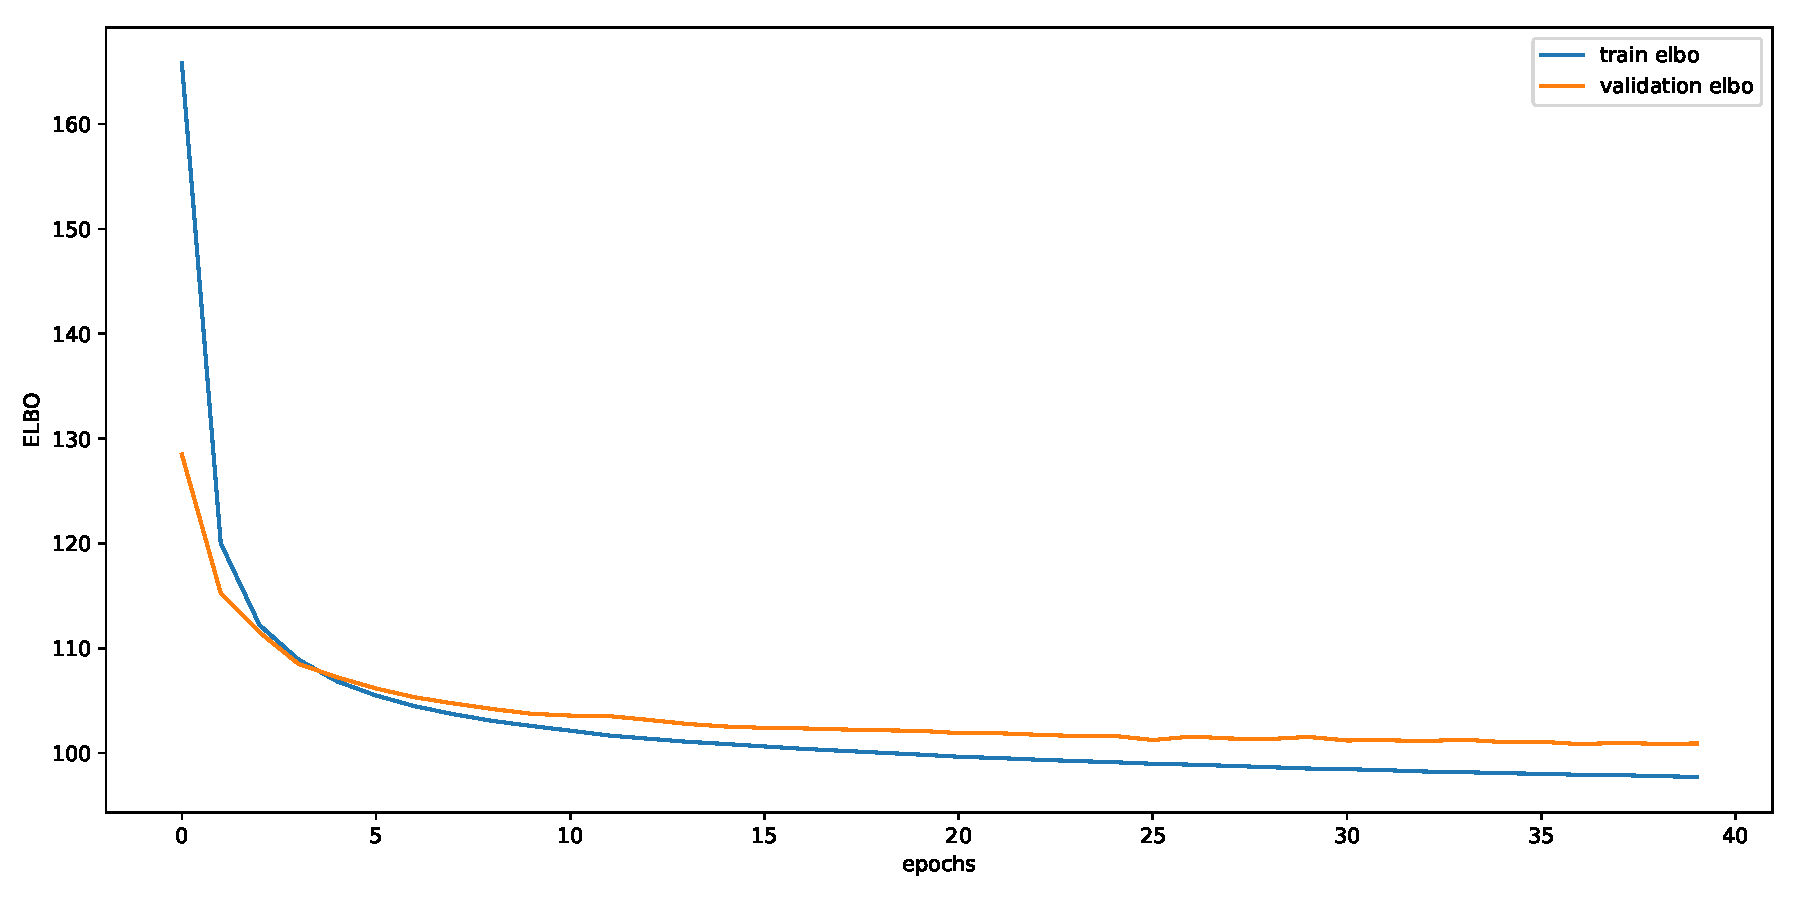
\includegraphics[width=\linewidth]{elbo.pdf}
        \caption{ELBO in VAE in 40 epochs}
        \label{fig:elbo_vae}
      \end{figure}
      \item Question 1.14 \\
      \begin{figure}[htbp]
        \centering
        \subfigure[]{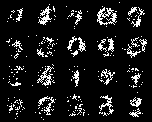
\includegraphics[width=0.3\textwidth]{VAE_EPOCH_0_20.png}}
        \subfigure[]{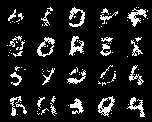
\includegraphics[width=0.3\textwidth]{VAE_EPOCH_20_20.png}}
        \subfigure[]{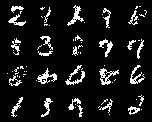
\includegraphics[width=0.3\textwidth]{VAE_EPOCH_39_20.png}}
        \caption{(a) First epoch (b) Midway epoch (c) Final epoch}
        \label{fig:progress_vae}
      \end{figure}
      \item Qeustion 1.15 \\
      \begin{figure}[H]
        \centering
        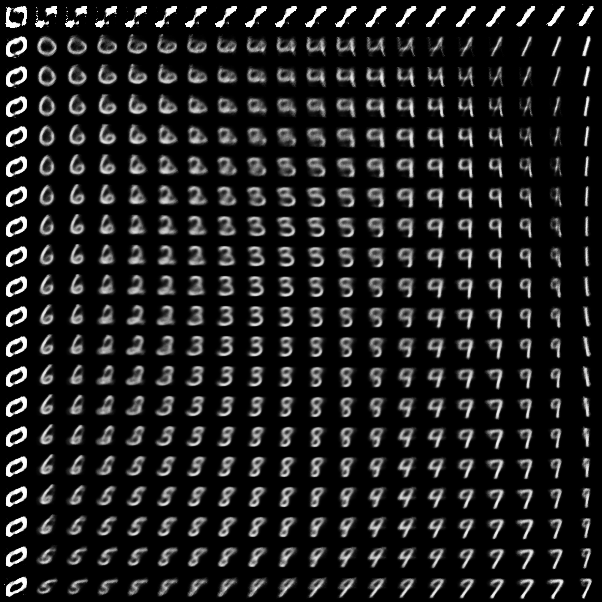
\includegraphics[width=\linewidth]{manifold.png}
        \caption{Manifold for a 2-dimensional latent space}
        \label{fig:manifold}
        As expected this manifold from \ref{fig:manifold} is not as clear as from the Figure \ref{fig:progress_vae} where a bigger $z$ latent space is used. This result coincide with the original paper, where a two dimensional latent space is not sufficient to approximate the probability of the data input, while higher values are. 
      \end{figure}
    \end{itemize}
\section{Generative Adversarial Networks}
    \begin{itemize}
      \item Question 2.1 \\
      For a generator we have random noise sampled from a distribution of choice which will generate a noisy image. This image together with the image of the training set will serve as input for the discriminator which will output labels , real or fake. Effectively the discriminator should discriminate well between the generator input and the data input. 
    \end{itemize}
    \subsection{Training objective: A minimax Game}
      \begin{itemize}
        \item Question 2.2 \\
        We want to deceive as well as possible the discriminator while maximize our classification power of the input data. So the generator wants to minimize its effect of the discriminator, while the discriminator wants to maximize its discriminative power over the generator. So the training objective is the sum of  the classification power of the discriminator and its discriminative power of the generator.
        \item Question 2.3 \\
        The value that will result after convergence with the minimax game between the generator and discriminator is  $-\log 4$ as when the discriminator cannot differentiate between \textbf{real} and \textbf{fake} it will have $\frac{1}{2} $ time to discern the labels. Combining this knowledge with equation 15, we obtain the sum of two times $-\log{2}$ which is $-\log{4}$ as stated before. 
        \item Question 2.4 \\
        This is the case because the discriminator is fairly certain that the generator is not the real data, the distribution generated from this generator is far from the underlying target distribution which is the image input. To solve this we rather maximize $D(G(Z))$ as this will give stronger gradients during back-propagation and thus learn faster how to fool the discriminator, so the aim is to increase the log probability of the discriminator to mistaken the generator input as the data input, rather to improve the generator impprove at discerning real from fake. The only difference with the previous emphasis is that $\mathrm{E}_{p_z(z)}\left[ \log \left( 1 - D(G(Z)) \right) \right]$ not quickly becomes $0$ thus not taking the adversiality into account. 
      \end{itemize}
    \subsection{Building GAN}
      \begin{itemize}
        \item Question 2.5 \\
        The GAN is implemented as proposed in the template. The non-linearity in the generator needs to be tahn as the distribution has to be between -1 en 1 while the discriminator has to be sigmoid activation function as it ouputs probabilities. The generator increases fast and clipping the norm did not solve the problem and using a batchnorm for the generator made the values converge quickly to NaN. Moreover the initialisation of the generator and discriminator has to actively pass the data otherwise nothing is processed. 
        \item Question 2.6  \\
        \begin{figure}[htbp]
          \centering
          \subfigure{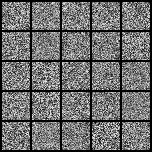
\includegraphics[width=0.3\textwidth]{0_0.png}}
          \subfigure{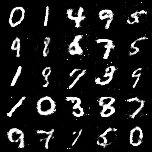
\includegraphics[width=0.3\textwidth]{100_94000.png}}
          \subfigure{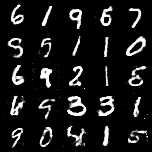
\includegraphics[width=0.3\textwidth]{199_187599.png}}
          \caption{Evolution of GAN zeroth epcochs, 100 epochs and final}
          \label{<label>}
        \end{figure}
        \item Question 2.7
      \end{itemize}
  \section{Generative Normalizing Flows}
      \subsection{Change of variables for Neural Networks}
        \begin{itemize} 
          \item Question 3.1 \\
          If the mapping of $f$ is an invertible smooth mapping and $x \in \mathbb{R}^m$ is a multivariate random variable then we will require the determinant of \textbf{Jacobian} of the input data instead of just the derivatives, formally:
          \begin{align*}
            z &= f(x); & x = f^{-1}(z); && p(z) = p( f^{-1}(z)) \det \Big| \frac{\partial f^{-1}}{\partial z} \Big| \\
            p(x) &= p(z) \det \Big| \frac{ \partial f}{\partial x} \Big|^{-1} & \text{change of variables}
          \end{align*} where $ \frac{ \partial f}{\partial x}$ is the Jacobian. Equivallently for our objective we will obtain the following:
          \begin{align*}
            \log p(x) &= \log p(z) + \sum_{l = 1}^{L} \log \det \Big| \frac{\partial h_l}{\partial h_{l -1}}\Big| \\
            &= p(z) +  \sum_{l = 1}^{L} \log \det \Big|J^TJ \Big|
          \end{align*} with $h_0 = x$ and $h_L = z$. 
          \item Question 3.2 \\
          This equation is computable if for each preceding dimensions the Jacobian is easily computed. Formally put, each preceding $h_{l-1}$ has to have a defined determinant and be invertible. 
          \item Question 3.3 \\
          Calculating $N \times N$ Jacobians are expensive operations which have complexity $O(N^3)$ which is not feasible for higher dimensional data. When we sample data depending of the complexity of the original data, the sampling may be fast or slow.
          \item Question 3.4 \\
          The consequence might be that the model will encourage degenerate solutions  that puts probability mass on discrete data points, so the representation of the true distribution of the original data is not entirely generated. To solve this \textbf{FLOW++} offered to add noise from an uniform distribution in the input data such that no probability mass is gathered around specific values. This change the discrete integers input to continuous random variables. 
        \end{itemize}
      \subsection{The coupling-layers of Real NVP}
        \begin{itemize}
          \item Question 3.5
          \begin{enumerate}
            \item Bijective mapping of input data
            \item Rate of transformation of data input depending on  a part of the data, in other words the Jacobian of some input of the data.
            \item This is the scaling of the input image conditioned on only previous data input and that in fact may be complex and this is the part of the neural network output.
            \item This is the determinant of every previous input data transformation, so this means it contains on its diagonal elements of scaling of a part of input data. 
            \item Because of the presence of the $\exp$ in the diagonal entries of the Jacobian and the restriction to be invertible the determinant of the Jacobian is positive indeed. 
            \item Taking the $\log$ is equivalent of taking the $\exp$ thus the diagonal entries of the Jacobian contains exponential term. 
            \item This is sampled input from the latent space and due to the fact that the set-up of the bijective function the backward computation of this statement is the reverse order of the original bijective function. 
          \end{enumerate}
        \end{itemize}
      \subsection{Building a flow-based model}
        \begin{itemize}
          \item Question 3.6  \\
          During training data input is conditioned, from a multivariate distribution to the product of one-dimensional conditional densities and are fed to the network, a part of the total image. In a recursive way the current input is fed through successive coupling layers with each layer alternating its input source from the previous conditioned data input which was left unchanged. After K layers the latent vector is obtained and its log-probability calculated from the latent distribution. This result is added to the sum of logged of the determinants to compute the negative log-likelihood of the input data, this will be taken as a loss and back-propagated. After training the the input may be another image or larger data set and the coupling layers will have classification power as each contains information of loss at a finer scale. The output will be a distribution of the representation of the input data. 
          \item Question 3.7 \\ 
          See code \begin{verbatim} a3_nf_template.py\end{verbatim}
          \item Question 3.8
          \begin{figure}[htbp]
            \centering
            \subfigure{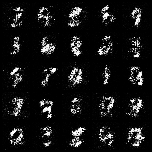
\includegraphics[width=0.3\textwidth]{nfs_0.png}}
            \subfigure[]{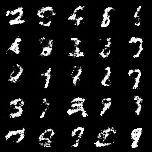
\includegraphics[width=0.3\textwidth]{nfs_20.png}}
            \subfigure[]{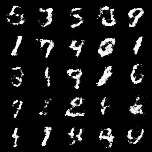
\includegraphics[width=0.3\textwidth]{nfs_39.png}}
            \caption{Evolution NF zeroth epoch halway and the end}
            \label{<label>}
          \end{figure}
        \end{itemize}
  \section{Conclusion}
        \begin{itemize}
          \item Question 4.1 \\
          We note that from alll the generative models, the GANs performs best producing clear images while the other two with much more computation the same could have been achieved. 
        \end{itemize}
    


\end{document}
